% !TeX program = xelatex
% !Mode:: "TeX:UTF-8"
%%  本模板推荐以下方式编译: xelatex
%%     1. 文件默认的编码为 UTF-8 对于windows,请选用支持UTF-8编码的编辑器。
%%   2. 若是模板有什么问题,请及时与我们取得联系,Email:latexstudio@qq.com。
%%   3. 可以到  https://ask.latexstudio.net 提问
%%   4. 请安装 最新版本的 TeXLive 地址:
%%   http://mirrors.ctan.org/systems/texlive/Images/texlive.iso

\documentclass[12pt,a4paper]{nmmcm}
\usepackage{ctex}
\usepackage{graphicx}
\usepackage{booktabs,colortbl}
\usepackage{xcolor}
\usepackage{tikz}
\usepackage{indentfirst}
\mcmsetup{CTeX = true,
        tcn ={\xiaowuhao 2024030125260 }, problem = C,
        sheet = true, titleinsheet = false, keywordsinsheet = true,
        titlepage = true, abstract = true}
\usepackage{xurl}
\setmainfont[
    Path=fonts/TimesNewRoman/,
    UprightFont = *-Regular,
    BoldFont = *-Bold,
    ItalicFont = *-Italic,
    BoldItalicFont = *-Bold-Italic  
]{TimesNewRoman}
\setmonofont[ 
    Path=fonts/UbuntuMono/,
    UprightFont = *-Regular,
    BoldFont = *-Bold,
    ItalicFont = *-Italic,
    BoldItalicFont = *-Bold-Italic  
]{UbuntuMono}
\usepackage{lipsum}

\usepackage{paralist}
\let\itemize\compactitem
\let\enditemize\endcompactitem
\let\enumerate\compactenum
\let\endenumerate\endcompactenum
\let\description\compactdesc
\let\enddescription\endcompactdesc

\setlength\abovedisplayskip{5pt}
\setlength\belowdisplayskip{-8pt}
\setlength{\parskip}{0.1em}

\newcommand\wordc[1]{\textbf{#1}}
\renewcommand{\appendixtocname}{附\quad录}
\renewcommand{\appendices}{\hspace{-2em}{\sanhao\HEI {\bf 附~~~录}}}
\colorlet{tableheadcolor}{gray!25} % Table header colour = 25% gray
\newcommand{\headcol}{\rowcolor{tableheadcolor}}

\title{\textcolor{red}{论文的题目(三号黑体)}}
\date{}

\usepackage[font=small,labelfont={bf,sf},tableposition=top]{caption}

% 我们团队自己的定制化操作
%%%%%%%%%%%%%%%%%%%%%%%%%%%%%%%%%%%%%%%%%%%%%%%%%%%%%%%%
\makeatletter
% 修改 section
\renewcommand\section{\@startsection{section}{1}{0pt}%
    {3.5ex plus 1ex minus .2ex}%
    {2.3ex plus .2ex}%
    {\normalfont\LARGE\bfseries}}
% 修改 subsection
\renewcommand\subsection{\@startsection{subsection}{2}{0pt}%
    {3.25ex plus 1ex minus .2ex}%
    {1.5ex plus .2ex}%
    {\normalfont\Large\bfseries}}
    % subsubsection标题的缩进
\renewcommand\subsubsection{\@startsection{subsubsection}{3}{1em}%
  {4ex plus 1ex minus .2ex}%
  {0.2ex plus .2ex}%
  {\normalfont\large\bfseries}}
\makeatother

\usepackage[backend=biber,style=gb7714-2015,gbfieldtype=true]{biblatex}
\addbibresource[location=local]{references.bib} 
%%%%%%%%%%%%%%%%%%%%%%%%%%%%%%%%%%%%%%%%%%%%%%%%%%%%%%%%%%%%

\begin{document}
\begin{abstract}
  

%abstract---------------
{\song\xiaosihao
\setlength{\parindent}{2em}\textcolor{red}{(第1段)	问题重述+简要思想:首先简要叙述所给问题的背景和动机,并分别分析每个小问题的特点(以下以三个问题为例)。根据这些特点说出自己的思想:针对于问题1,采用~$\cdots \cdots$ 的方法解决;针对问题2用~$\cdots \cdots$ 的方法解决;针对问题3用~$\cdots \cdots$ 的方法解决。}


\setlength{\parindent}{2em}\textcolor{red}{(第2段)	模型建立及求解结果:介绍思想和模型: 对于问题1我们首先建立了~$\cdots \cdots$ 模型I。首先利用~$\cdots \cdots$ ,其次计算了~$\cdots \cdots$ ,并借助~$\cdots \cdots$ 数学算法和~$\cdots \cdots$ 软件得出了~$\cdots \cdots$ 结论。}

\setlength{\parindent}{2em} \textcolor{red}{(第3段)	对于问题2我们用~$\cdots \cdots$(模型的建立与求解结果的陈述中,思想、模型、软件和结果必须描述清晰,亮点详细说明需突出。}

\setlength{\parindent}{2em}\textcolor{red}{(第4段)	对于问题3我们用~$\cdots \cdots$ (模型的建立与求解结果的陈述中,思想、模型、软件和结果必须描述清晰,亮点详细说明需突出。}

\setlength{\parindent}{2em}\textcolor{red}{(第5段)	优化结果及总结:在~$\cdots \cdots$ 条件下,针对~$\cdots \cdots$ 模型进行适当修改与优化,这种条件的改变可能来自你的一种猜想或建议。要注意合理性。此推广模型可以不深入研究,也可以没有具体结果。}
}

\begin{rmk}
    字数300$\sim $600之间,需控制在一页;摘要中必须将具体方法、模型和所得结果写出来;摘要要求“总分总”,段开头可用“针对问题1,针对问题2,针对问题3..”或者“首先,然后,其次,最后”等词语进行有逻辑的论述。摘要是重中之重,必须严格执行!
\end{rmk}







  \begin{keywords}
    {\song\xiaosihao
      \textcolor{red}{使用到的模型名称、方法名称、特别是亮点一定要在关键字里出现,3$\sim$ 5个较合适。}}
  \end{keywords}

  \begin{itemize}
    \item \textcolor{blue}{前面一页必须使用模板格式(黑色部分),否则论文检测不通过。}
    \item \textcolor{blue}{ 目录页为论文开始处,论文正文用阿拉伯数字从“1”开始连续编号,页码位于每页页脚中部。(鼓励使用目录)}
  \end{itemize}

\end{abstract}
\maketitle
\renewcommand{\contentsname}{\centerline{\sanhao\bfseries\HEI 目\quad 录}}
%\thispagestyle{empty}
%{\song\xiaosihao
\tableofcontents
%}

\newpage
\setcounter{page}{1}
\pagestyle{fancy}
\section{问题重述}
本研究针对天然气水合物(Natural Gas Hydrate/Gas Hydrate),即通常所称的“可燃冰”,这是一种在特定高压低温环境下与水结合形成的类冰状结晶物质。由于其外观类似冰块且能在火源接触下燃烧,故此得名。这种物质主要分布在深海沉积物或陆地的永久冻土层中,是一种被国际能源领域高度重视的潜在清洁能源。
在能源科学研究与勘探领域中,天然气水合物的勘探和量化评估是一项复杂且技术要求高的任务。其关键挑战包括但不限于:资源的空间定位、量化评估、经济可行性分析以及对气候变化的潜在影响评价。当前,虽然天然气水合物被视为替代传统石油和天然气资源的重要选择,但相关的资源勘探和评估技术仍显不足,尤其是在资源量的精确计算和预测方面。
对于天然气水合物资源量的估计主要依赖两种思路:成藏思路和生烃思路。成藏思路方法着眼于天然气水合物的赋存状态,通过确定天然气水合物的聚集区域并评估其规模和数量分布来估计资源量。而生烃思路方法则从有机质的沉积和演化过程出发,通过物质守恒原理模拟水合物的生成和运聚过程。在实际应用中,成藏思路的体积法由于其直观性和适用性较广,成为了评估天然气水合物资源量的主流方法。
在本研究中,依据地质资源勘探部门在特定海域内的14个钻孔勘探数据,这些数据包括每个钻孔的具体位置、深度以及相应深度的孔隙度和天然气水合物饱和度的测量信息。本研究旨在:
\begin{enumerate}
  \item 确定研究区域内天然气水合物的资源分布范围;
  \item 评估区域内资源参数如有效厚度、地层孔隙度和饱和度的概率分布及其变化规律;
  \item 基于统计分析提出天然气水合物资源量的概率分布估计;
  \item 针对资源评估的进一步精细化,提出在研究区域增加钻探井位的策略。
\end{enumerate}

\subsection{引言}
%Introduction---------------

\setlength{\parindent}{2em} 
在本研究中,依据地质资源勘探部门在特定海域内的14个钻孔勘探数据,这些数据包括每个钻孔的具体位置、深度以及相应深度的孔隙度和天然气水合物饱和度的测量信息。本研究旨在:

1)确定研究区域内天然气水合物的资源分布范围;

2)评估区域内资源参数如有效厚度、地层孔隙度和饱和度的概率分布及其变化规律;

3)基于统计分析提出天然气水合物资源量的概率分布估计;

4)针对资源评估的进一步精细化,提出在研究区域增加钻探井位的策略。

\subsection{要解决的具体问题}
\begin{enumerate}
  \item
        问题一:问题1的重述,重述语言简洁明了,突出模型中第一个要解决的问题,突出核心。
  \item
        问题二:问题2的重述。
  \item
        问题三:问题3的重述。
  \item
        问题四:问题4的重述。
\end{enumerate}


\section{问题分析}
\subsection{问题1的分析}

对问题1研究的意义的分析。
问题1属于$\cdots\cdots$数学问题,对于解决此类问题一般数学方法的分析。
对附件中所给数据特点的分析。
对问题1所要求的结果进行分析。
对问题1研究的意义的分析。


\subsection{问题2的分析}
问题2属于$\cdots\cdots$数学问题,对于解决此类问题一般数学方法的分析。
对附件中所给数据特点的分析。
对问题2所要求的结果进行分析。
由于以上原因,我们可以将首先建立一个$\cdots\cdots$的数学模型I,然后将建立一个$\cdots\cdots$的模型II,$\cdots\cdots$对结果分别进行预测,并将结果进行比较.


\subsection{问题3的分析}
问题1属于$\cdots\cdots$数学问题,对于解决此类问题一般数学方法的分析。
对附件中所给数据特点的分析。
对问题1所要求的结果进行分析。
对问题1研究的意义的分析。

\subsection{问题4的分析}
问题4属于空间优化和资源分配的数学问题。
在解决此类问题时,通常需要采用多目标优化方法来平衡不同的优化目标。
本问题中,需要在保证新井位置的离散性的同时,最大化这些新井所能探测到的总资源量。


\section{模型假设}
\begin{enumerate}
  \item 假设题目所给的数据真实可靠,无错误记录数据。
  \item 在计算每个位置点的水合物资源量,我们假设所有位置点的检测数据和其周围单位体积内的位置点数据相同 $A \times Z$($\text{有效面积} \times \text{单位厚度}$)。
  \item 假设具有天然气特性的物质排除天然气以外的任何物质,地壳内不存在其他混淆干扰物,天然气水合物在研究区域内呈连续分布,没有断层或其他地质障碍导致的断裂。
  \item 假设观测期内储层参数保持稳定,研究区域内的地质结构相对均质,在勘探和开发周期内,天然气水合物的赋存状态不会因外界因素(如温度、压力变化)而发生显著变化。不受其他因素影响
  \item 在处理孔隙度、饱和度等参数的统计数据时,假定各钻孔点的数据相互独立。这意味着每个数据点提供的信息是独立的,没有因地理位置或地质联系而产生的相关性。
\end{enumerate}

\section{名词解释与符号说明}

\subsection{名词解释与说明}
\begin{enumerate}
  \item \wordc{有效厚度:}
        是指储油层中具有工业产油能力的那部分油层的厚
        度,即工业油井内具可动油的储集层的厚度。有非 0 饱和度的点存在
        天然气水合物。
  \item \wordc{水合物饱和度:}
        单位体积大矿物质中水合物所占的体积分
        数。
  \item \wordc{产气量因子:}
        指 1 立方米天然气水合物能量相当于多少立方
        米的天然气的热值。
  \item \wordc{粒子群优化算法(PSO):}
        是一种基于群体智能的优化工具,通过模拟鸟群的社会行为来寻找问题的最优解。
        算法中,每个“粒子”代表解空间中的一个潜在解,它们根据个体和群体的经验来调整自己的位置,以寻找最优解。
  \item \wordc{Kriging插值法:}
        是一种基于统计学的空间插值技术,广泛用于地质统计和空间分析。
        该方法利用变异函数来评估空间数据点之间的相关性,从而预测未知位置的值,
        优势在于能够提供插值误差估计,从而增强插值结果的可靠性。
\end{enumerate}


\subsection{主要符号与说明}

%tab1
\begin{table}[h!]
  \centering
  \small
  \begin{tabular}{p{60pt}<{\centering}|p{60pt}<{\centering}p{180pt}<{\raggedright}}
    \hline
    \headcol 标号 & 符号       & 符号说明(定义)              \\
    \hline
    Q           & $Q$      & 天然气水合物资源量 (m$^2$)     \\
    A           & $A$      & 表面面积   (m$^2$)        \\
    Z           & $Z$      & 有效厚度                  \\
    $\phi$      & $\phi$   & 孔隙度                   \\
    S           & $S$      & 水合物饱和度                \\
    E           & $E$      & 产气量因子                 \\
    $x_i$       & $x_i$    & 第 $i$ 个位置点的横坐标   (m)  \\
    $y_i$       & $y_i$    & 第 $i$ 个位置点的纵坐标   (m)  \\
    $z_i$       & $z_i$    & 第 $i$ 个位置点的高度   (m)   \\
    $\phi_i$    & $\phi_i$ & 第 $i$ 个位置点的孔隙度        \\
    $S_i$       & $S_i$    & 第 $i$ 个位置点的水合物饱和度     \\
    $Q_i$       & $Q_i$    & 第 $i$ 个位置点的水合物资源量    \\
    $x_j$       & $x_j$    & 第 $j$ 个勘探井位的横坐标   (m) \\
    $y_j$       & $y_j$    & 第 $j$ 个勘探井位的纵坐标   (m) \\
    $Q_j$       & $Q_j$    & 第 $j$ 个勘探井位的水合物资源量    \\
    \hline
    \hline
  \end{tabular}
  %\caption{符号与说明}
  \label{tab:symbol}
\end{table}


\section{模型的建立与求解}

\subsection{数据的预处理}:
根据题目需求描述,我们需要对每个井位下的天然气水合物含量、有效厚度、饱和度、概率分布等变化规律进行分析与建模,附件一和附件二提供了钻井测量数据,井位信息,但数据存在部分误差,以及失访情况下造成的数据缺失,需要对原始数据进一步处理方可使用。
\begin{enumerate}
  \item 格式标准化:为确保数据处理的一致性和后续分析的顺利进行,我们手动对所提供数据的分隔符进行了统一。具体操作主要有三:将数据中的分隔符不统一问题统一转换为制表符;将原始数据文件的编码格式由GDK转换为UTF-8编码防止出现读取乱码问题;所有文件按照英文命名规则进行重命名。
  \item 读取所有数据,用空值替换掉缺失值。
  \item 异常值剔除
        孔隙度是指岩石中孔隙空间的体积与岩石总体积的比值,它是衡量岩石多孔性的一个重要参数,通常用小数或百分比表示。含水合物饱和度是指在岩石孔隙空间中,天然气水合物所占的体积与孔隙总体积的比值。在附件一中,孔隙度和含水合物饱和度出现了理论范围内的正常值和负值。由于负值是异常,
        基于负值的计算会使得资源量出现负值,但是考虑到数据具体测量方式未知,试探性使用 Min Max 标准化方法,将数据序列按照大小映射到 [0,1] 区间
        %公式:处理结果/图:
        我们发现,尽管该方法能够消除负值,但同时也导致了数据的过度失真。标准化后的数据丧失了原有的地质学意义,决定不采用Min-Max标准化方法。
        最后对原始数据集中出现的负数值全部进行了识别和排除。
        %处理后的数据如下:
\end{enumerate}
\subsection{问题1的分析和求解}

\subsubsection{问题1模型的建立}

\subsubsection{问题2模型的求解}

将预处理数据带入上述模型,通过$\cdots$软件得到$\cdots$结果。(编程代码详见附件*)。模型求解及结果需要图文并茂,用数据说话  用图展示。具体步骤123$\cdots$
\begin{align}
  A_{\max} & =\dfrac{3600}{t_{\min}}=\dfrac{3600}{J_{\min} /(v / 3.6)}
  =\dfrac{1000 v}{J_{\min }}(\text{辆 } / h)                            \\
  J_{\min} & =J_{\rm r}+J_{z}+J_{\rm a}
\end{align}


\subsubsection{问题2结果}




\subsection{问题3模型的建立和求解}

\subsubsection{问题3模型的建立}
对于资源量的概率分布估计,我们沿用了问题2中的 KDE 方法,通过核密度估计来估计资源量的概率分布。




\subsection{问题4模型的建立和求解}
\subsubsection{二维 Kriging 插值模型的建立}
二维 Kriging 插值是一种高级的地统计学方法,用于预测空间数据的分布。在本研究中,我们使用普通Kriging模型(Ordinary Kriging)来估计未知位置的资源量,基于已知井点的资源数据。

\begin{enumerate}
  \item \textbf{数据准备和预处理} \\
        首先,我们从已有的井点数据中提取坐标 $(x_i, y_i)$ 和对应的资源量 $z_i$。这些数据点作为Kriging插值的输入,用于构建空间连续性模型。

  \item \textbf{普通Kriging模型} \\
        普通Kriging模型的基本公式可以表示为:
        \[
          Z(x) = \mu + \sum_{i=1}^n \lambda_i (Z(x_i) - \mu)
        \]
        其中,$Z(x)$ 是在位置 $x$ 的预测值,$\mu$ 是未知常数(通常是全局均值),$Z(x_i)$ 是已知数据点的值,$\lambda_i$ 是权重系数,$n$ 是用于预测的已知数据点的数量。

  \item \textbf{变异函数和模型参数} \\
        在Kriging方法中,变异函数(semivariogram)是描述空间数据点之间关系的关键。在本研究中,我们选择球形变异函数模型,其表达式为:
        \[
          \gamma(h) =
          \begin{cases}
            C_0 + C \left( \frac{3h}{2a} - \frac{h^3}{2a^3} \right) & \text{if } h \leq a \\
            C_0 + C                                                 & \text{if } h > a
          \end{cases}
        \]
        其中,$h$ 是空间距离,$C_0$ 是块金效应(nugget effect),$C$ 是基台值(sill),$a$ 是变程(range),即空间相关性的最大距离。

  \item \textbf{权重系数的确定} \\
        权重系数 $\lambda_i$ 通过解决Kriging方程来确定,确保预测误差最小化。Kriging方程可以表示为:
        \[
          \sum_{j=1}^n \lambda_j \gamma(x_i, x_j) + \mu = \gamma(x_i, x)
        \]
        对于所有 $i = 1, 2, \ldots, n$。此外,为了保证无偏估计,权重的和应该满足:
        \[
          \sum_{i=1}^n \lambda_i = 1
        \]

  \item \textbf{插值和预测} \\
        最后,使用解得的权重系数 $\lambda_i$ 和模型参数,我们可以计算任意位置 $x$ 的资源量预测值 $Z(x)$。这一过程涉及到在整个研究区域内创建一个平面网格,并在每个网格点上应用上述Kriging公式进行资源量预测。
\end{enumerate}

\subsubsection{二维 Kriging 插值模型的求解}

\begin{enumerate}
  \item \textbf{实验半方差图结果分析} \\
        如图 \ref{fig:KrigingSemivariogram} 所示,实验半方差图显示了理论模型(黑色曲线)与实际观测数据点(红色星号)的对比。主要观察结果包括:
        \begin{itemize}
          \item 实际数据点大体上遵循理论模型的趋势,表明所选的球形变异函数模型是合适的。
          \item 在较小的空间距离 \( h \) 上,数据点与理论曲线较为接近,说明在小范围内,空间自相关性较强。
          \item 随着 \( h \) 的增加,实际数据点的分布开始波动,可能反映了在较大距离上空间自相关性的减弱。
        \end{itemize}

        % Insert pics
        \begin{figure}[h]
          \centering
          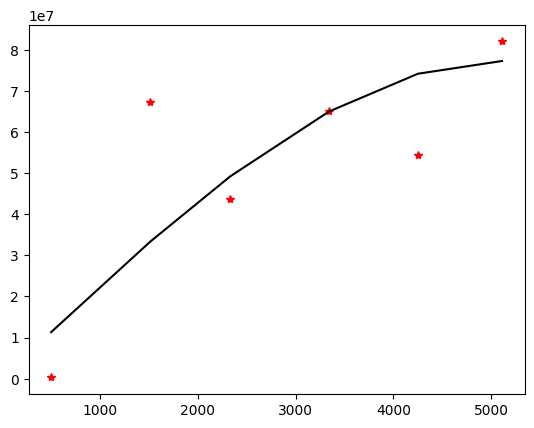
\includegraphics[width=0.5\textwidth]{figures/task4/task4-1.png}
          \caption{实验半方差图结果}
          \label{fig:KrigingSemivariogram}
        \end{figure}


  \item \textbf{预测误方差与插值结果分析} \\
        第二张图片(图 \ref{fig:KrigingInterpolation})展示了 Kriging 预测的方差(左图)和资源量的插值结果(右图)。分析如下:
        \begin{itemize}
          \item \textbf{预测误方差图(左图)}:
                \begin{itemize}
                  \item 显示了各个位置的预测误差大小,颜色越亮(趋向黄色)表示预测的不确定性越大。
                  \item 在已知数据点附近,预测误差较小,显示模型在数据点附近具有较高的信度。
                  \item 数据点间的区域预测误差增大,反映了这些区域内插值的不确定性较高。
                \end{itemize}
          \item \textbf{资源量插值结果图(右图)}:
                \begin{itemize}
                  \item 此图显示了整个区域的资源量预测分布。颜色越亮(趋向黄色)表示预测的资源量越高。
                  \item 资源量的高值区主要集中在某些特定区域,可能与原始数据点的分布和地质特性有关。
                  \item 插值结果显示了资源分布的空间变异性,有助于理解资源在研究区域内的分布特征。
                \end{itemize}
        \end{itemize}
        \begin{figure}[h]
          \centering
          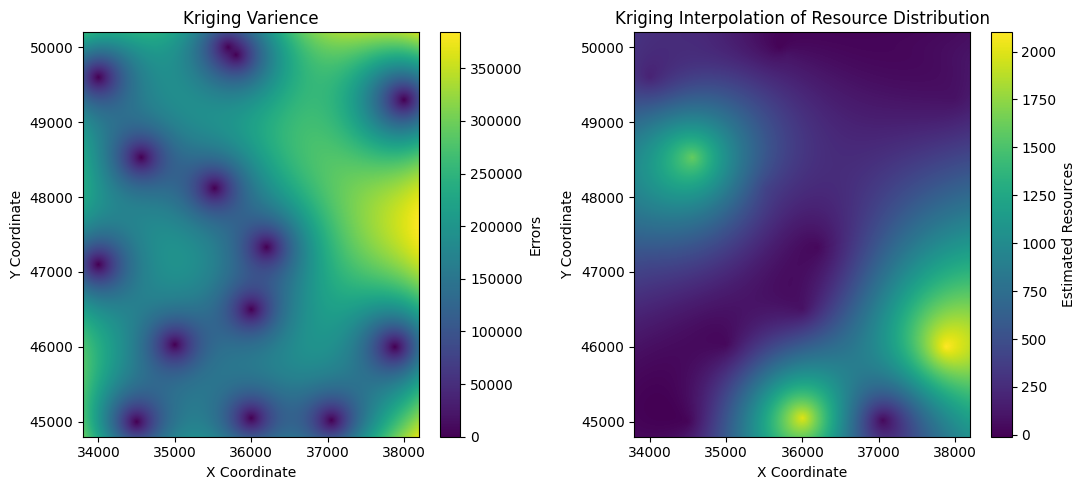
\includegraphics[width=0.8\textwidth]{figures/task4/task4-2.png}
          \caption{预测误方差(左)和 插值结果(右)}
          \label{fig:KrigingInterpolation}
        \end{figure}
\end{enumerate}



\subsubsection{粒子群优化算法的数学模型}
粒子群优化(PSO)是一种基于群体的优化技术,模拟鸟群的社会行为来寻找问题的最优解。每个粒子代表潜在的解决方案,在解空间中按照简单的数学规则移动。

\begin{enumerate}
  \item \textbf{粒子的表示} \\
        在PSO中,粒子$i$在$d$维搜索空间中的位置表示为$\mathbf{x}_i = (x_{i1}, x_{i2}, \ldots, x_{id})$,速度表示为$\mathbf{v}_i = (v_{i1}, v_{i2}, \ldots, v_{id})$。每个粒子还维护一个个人最优位置$\mathbf{p}_{\text{best},i}$,即该粒子历史上遇到的最优位置。

  \item \textbf{速度和位置更新} \\
        粒子的速度和位置通过以下公式更新:
        \[
          \mathbf{v}_i^{(t+1)} = w \mathbf{v}_i^{(t)} + c_1 r_1 (\mathbf{p}_{\text{best},i} - \mathbf{x}_i^{(t)}) + c_2 r_2 (\mathbf{g}_{\text{best}} - \mathbf{x}_i^{(t)})
        \]
        \[
          \mathbf{x}_i^{(t+1)} = \mathbf{x}_i^{(t)} + \mathbf{v}_i^{(t+1)}
        \]
        其中,$w$是惯性权重,控制粒子速度的保留程度;$c_1$和$c_2$是学习因子,通常称为认知和社会参数;$r_1$和$r_2$是[0,1]区间内的随机数,代表随机性;$\mathbf{g}_{\text{best}}$是全局最优位置,即所有粒子历史上遇到的最优位置。

  \item \textbf{参数选择} \\
        惯性权重$w$通常设置为0.7至0.9之间,有助于控制搜索的全局和局部探索能力。学习因子$c_1$和$c_2$通常设置为相同的值,比如1.5,这样可以平衡个体经验和群体经验的影响。

  \item \textbf{初始化和迭代过程} \\
        每个粒子的初始位置和速度通常是随机生成的。在每次迭代中,根据上述规则更新所有粒子的速度和位置。同时,更新每个粒子的个人最优位置以及全局最优位置。迭代继续进行,直到满足最大迭代次数或其他终止条件。

  \item \textbf{目标函数和优化目标} \\
        PSO目标是找到使目标函数$J(x)$最大化的解$\mathbf{x}$。在本文中,目标函数是最大化新井位置的预测资源总量和最小化井点间的最短距离的负值。
\end{enumerate}


\subsubsection{基于 Kriging 插值的优化模型建立}

在 Kriging 模型的求解结果和粒子群优化算法的基础上,我们进一步建立了一个优化模型,旨在确定新井的最佳位置,以最大化资源的总探测量和井点之间的距离。模型的目标函数综合考虑了新井之间以及新旧井之间的最小距离和新井位置的预测资源总量。

\begin{enumerate}
  \item \textbf{目标函数定义} \\
        设计目标函数如下,用于评估新井布置的质量:
        \[
          J(x) = -\left(\min(\text{dist}(x_i, x_j)) + \sum_{k=1}^{n} Z(x_k, y_k)\right)
        \]
        其中,$n$ 为新井的数量,$x = \{(x_1, y_1), (x_2, y_2), \ldots, (x_{n}, y_{n})\}$ 表示新井的位置,$\text{dist}(x_i, x_j)$ 表示所有井点(包括现有和新井)之间的欧氏距离矩阵,$Z(x_k, y_k)$ 是在位置 $(x_k, y_k)$ 的预测资源量,通过 Kriging 插值得到。

  \item \textbf{优化算法选择} \\
        我们采用粒子群优化(PSO)算法来解决这一多目标优化问题。PSO 是一种基于群体的随机优化技术,通过模拟鸟群的社会行为来搜索最优解。在本问题中,每个粒子代表一组潜在的新井位置,粒子通过迭代更新其位置,以寻找使目标函数最大化的解。

  \item \textbf{粒子群优化参数设置} \\
        在 PSO 算法中,我们设置了如下参数:个体学习因子$c_1$、社会学习因子$c_2$和惯性权重$w$。这些参数控制粒子更新其速度和位置的方式,其中$c_1$和$c_2$通常设置为1.5,$w$设置为0.7。

  \item \textbf{约束条件和边界} \\
        新井的位置受到现有井位置的范围约束,即每个新井的坐标$(x, y)$必须在现有井的最小和最大坐标范围内。这确保了新井的位置在合理的探测区域内。

  \item \textbf{优化执行} \\
        优化过程包括初始化一定数量的粒子,每个粒子代表一组新井的位置。通过迭代,每个粒子根据其自身经验和群体经验更新位置,直到达到最大迭代次数或满足其他终止条件。最终,算法输出最优的新井位置和相应的目标函数值。
\end{enumerate}

\subsubsection{优化模型的求解}
在本节中,我们将详细分析基于Kriging插值和粒子群优化算法(PSO)建立的优化模型的求解结果。该模型的目标是确定新井的最佳位置,以最大化资源的探测量并优化井点之间的距离。
\begin{enumerate}

  \item \textbf{新井位置优化结果}

        首先,我们从新井的布局开始。如图 \ref{fig:NewWellsAndOldWells} 所示,新井(红色点)与现有井(蓝色点)的布局展示了新井的选址策略不仅考虑了资源量的最大化,同时也确保了合理的空间分布,避免过于集中或偏远。

        \begin{figure}[h]
          \centering
          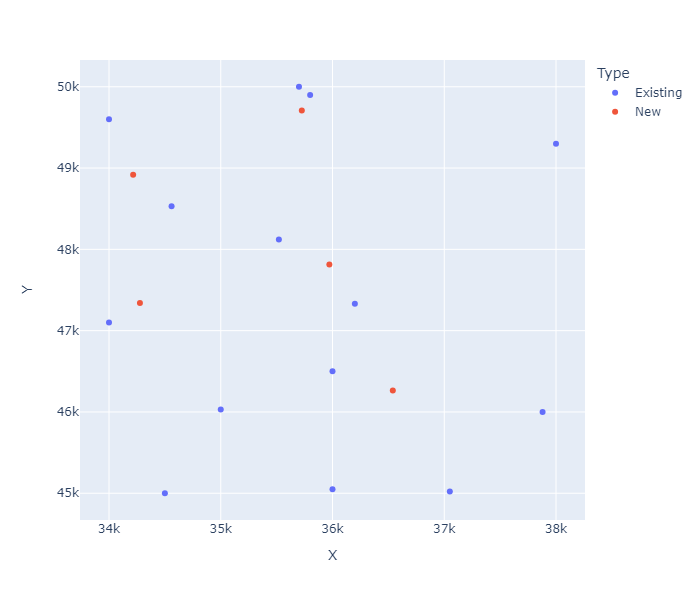
\includegraphics[width=0.5\textwidth]{figures/task4/task4-3.png}
          \caption{新井位置优化结果}
          \label{fig:NewWellsAndOldWells}
        \end{figure}

  \item \textbf{资源量和不确定性分析}

        接下来,我们通过Kriging插值的结果来分析资源量分布和不确定性。如图 \ref{fig:NewWellsAndResource} 右侧所示,Kriging插值的资源分布图显示了预测的资源量,其中颜色越暗表示资源量越高。这帮助我们验证新井位置的选择是否位于资源丰富的区域。左侧的Kriging方差图表则提供了关于预测不确定性的信息,颜色越亮表示不确定性越高,这通常出现在样本点较少的区域。

        \begin{figure}[h]
          \centering
          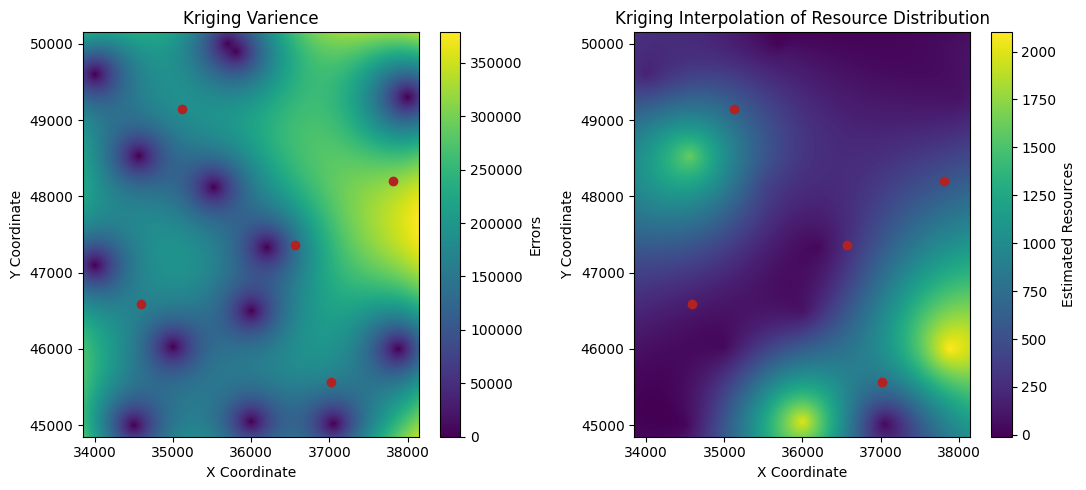
\includegraphics[width=0.8\textwidth]{figures/task4/task4-4.png}
          \caption{新井位置资源量情况}
          \label{fig:NewWellsAndResource}
        \end{figure}

  \item \textbf{井点距离的离散程度分析}

        最后,我们分析了添加新井前后所有井点距离的离散程度。如图 \ref{fig:NewWellsAndNoNewWells} 所示,通过箱型图和小提琴图可以看出,引入新井后,井点之间的距离的中位数有所降低,这表明新井的加入使得井点分布更加均匀。小提琴图进一步揭示了数据分布的密度和范围,展示了新井引入前后井点距离分布的变化。

        \begin{figure}[h]
          \centering
          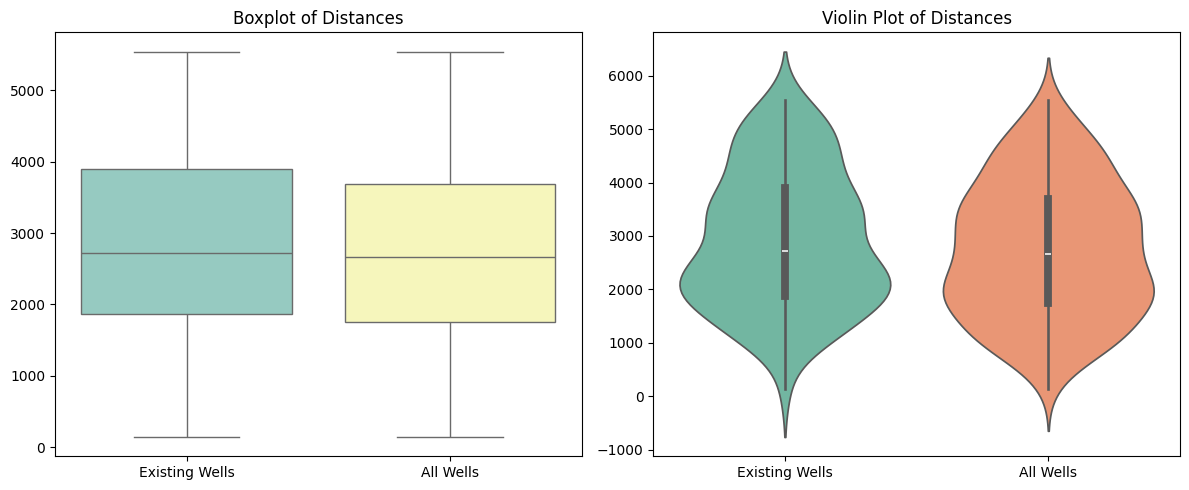
\includegraphics[width=0.8\textwidth]{figures/task4/task4-5.png}
          \caption{添加新井前后,所有井距离的离散程度}
          \label{fig:NewWellsAndNoNewWells}
        \end{figure}
\end{enumerate}


\section{模型的评价与推广 模型的评价与推广}

\textcolor{red}{将模型进行数值计算,并与附件中的真实采样值(进行列表或图示)比较。对误差进行数据分析,给出误差分析的理论估计。}

\subsection{模型的评价}


1. 优点

\textcolor{red}{得到满意的解、
  较好地解决了$\cdots$问题、
  使模型得到简化、
  使结果更合理,避免…带来的较大误差、
  使问题描述比较清晰、
  减少大的计算量。
}

(1)问题求解中 辅之流程图, 将建模思路完整清晰的展现出来;

(2)问题二在对 问题二在对理论通行能力进修复时考虑因素 细致、全面,理论通行能力进修复时考虑因素
细致、全面,系数准确度高;

(3)在问题三中,提出“影响度”的概念较为直观地定量给小区开放后的效果,简便有.在影响度计算上由
点及面从每个路段、交叉口到整 个路网,层深入具有逻辑性;


(4)运用多种数学软件(如 MATLAB、SPSS),取长补短,使计算结果更加),取长补短,使计算结果更
加 准确、明晰.

2. 缺点

\textcolor{red}{主观性过强、
  建立在什么的前提条件下、
  有一定的局限性、
  存在不确定性、
  有一定的偏差。
}

(1)在数学软件的计算中会将小数计算 结果进行保留,使得随后的会将小数计算 结果进行保留,使得随后
的或统计结果造成一定误差;

(2)问题二求解修正通行能力时多次使用了查表,操作不够简便.

\subsection{模型的、模型的 推广}

\begin{itemize}

  \item \textcolor{red}{对本文中的模型给出比较客观的评价,必须实事求是,有根据,以便评卷人参考。}

  \item \textcolor{red}{推广和优化,需要花费功夫想出合理的、甚至可以合理改变题目给出的条件的、不一定可行但是具有一定想象空间的准理想的方法、模型。由此做出一些改进方向,也可以是参赛者一些来不及实现的思路。}
\end{itemize}

1. 问题二中 建立 的模型 在现实 生活 中可以 作为 检验 数据 对实测数据 的准确 性进行 检验,帮助 人们
更好 的测算 交通 数据.

2. 基于问题三建立的模型,可以根据道路实时检测数(某段单位间内 基于问题三建立的模型,推算新建
一条道路对于当前交 通状况的改善效果,帮助度等).

\section{模型的改进}

\subsection{模型一的改进}
针对问题二中的模型一,在具体求解大型车对车辆通行能力的修正系数时,
我们利用交通量的测算值对照得到相应的大型车修正系数.但是,在实际操作中
交通量的测定有很大的难度,如果此时交通量数据无法得到,那么我们便不能得
到相应的修正系数,因此我们对模型进行改进.

由~GREENSHIELD K-V 线性模型,可得通行能力的公式:
\begin{align}
  A_{p}=\begin{cases}
          \dfrac{3600}{t}\left(1-\dfrac{3.6 l}{V_{t} t}\right)\left(V_{f}>7.2 l / t\right) \\
          \dfrac{250 V_{f}}{t}\left(V_{f} \leq 7.2 l / t\right)
        \end{cases}
\end{align}

对应的临界车辆速度:
\begin{align}
  V_{p}=\begin{cases}
          \dfrac{V_{f}-3.6 l}{t} & \left(V_{f}>7.2 l / t\right)      \\
          \dfrac{1}{2} V_{f}     & \left(V_{f} \leq 7.2 l / t\right)
        \end{cases}
\end{align}

由美国道路通行能力准则可得,美国将道路服务水平分为六级:A-F 级,而
我国目前针对当前国情,将道路服务水平分成四级:一级相当于美国的A、B 两
级;二级相当于美国的C 级;三级相当于美国的D 级;四级相当于美国的E、F
级。因此,相应的,将美国服务水平划分标准进行针对性修正,得到中国道路服
务水平划分标准,见表

\begin{table*}[h!]
  \centering
  \small
  \tabcolsep 2pt
  \caption{我国服务水平划分标准}
  \begin{tabular*}{0.87\linewidth}{p{60pt}<{\centering}p{40pt}<{\centering}
    p{40pt}<{\centering}p{40pt}<{\centering}p{40pt}<{\centering}
    p{80pt}<{\centering}p{40pt}<{\centering}}
    \toprule
    服务水平 (L0S)  & \multicolumn{2}{c} {一级 } & 二级  & 三级  & \multicolumn{2}{c} {四级 } \\
    \cline{2-3}\cline{6-7}
    服务交通量  & 800 & 1200 & 1800 & 2500 & $A_{D}$ & $\leqslant A_{P}$ \\
    速度  km / h & 120 & 120 & 120 & 120 & $\geqslant V_{p}$ & $\leqslant V_{p}$ \\
    V / C & 0.33 & 0.48 & 0.71 & 1.0 & $A_{p} / A_{\max}\leqslant 1.0$ & -(无意义 ) \\
    \bottomrule
  \end{tabular*}
\end{table*}

由于车流量的测算相对于交通量来说较易得到,我们便可以不用对交通量进
行测算,可以通过车流量与通行能力的比值计算出~V/C 饱和度值,再通过该值对
照我国服务水平划分标准,间接得到服务交通量,从而得到大型车对通行能力的
修正系数.


\subsection{模型二的改进}

针对于问题三中的模型,在得出各个类型小区在开放后对于整个小区周边路
网交通负荷影响度后,无法判别小区开放的效果是积极的还是消极的,由此我们
可以采用~Bress 悖论的原理进行判别:在个人独立选择路径的情况下,为某路网
增加额外的通行能力(如增加路段的等),反而会导致整个路网的整体运行水平
降低的情况.

将路网进行简化如图~15:

根据推导可得: 当 $\beta_{3}/\left(\beta_{1}+\beta_{2}\right) \leq\left(\beta_{5}+\beta_{6}\right)/\beta_{4}$ 时,会发生悖论,即道路的开
通反而会加剧原有道路的交通状况.



\newpage

\nocite{*}
\printbibliography

\newpage

\begin{appendices}

\end{appendices}
\end{document}
%%
%% This work consists of these files mcmthesis.dtx,
%%                                   figures/ and
%%                                   code/,
%% and the derived files             mcmthesis.cls,
%%                                   mcmthesis-demo.tex,
%%                                   README,
%%                                   LICENSE,
%%                                   mcmthesis.pdf and
%%                                   mcmthesis-demo.pdf.
%%
%% End of file `mcmthesis-demo.tex'.
